\chapter{Provedené experimenty}

\section{Bludiště}

\begin{figure}
  \centering
  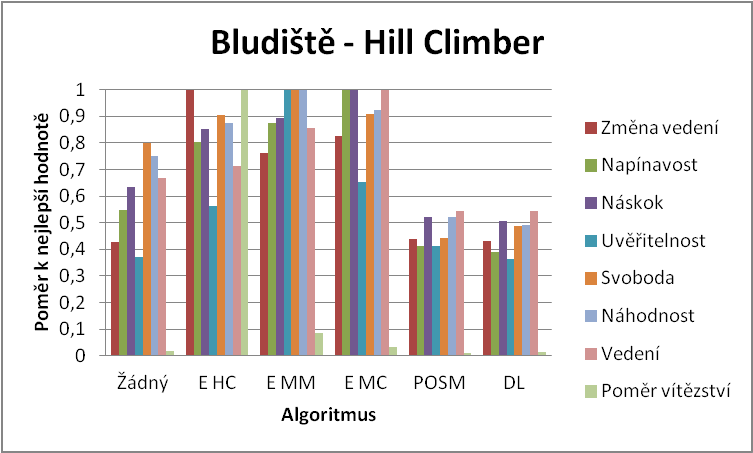
\includegraphics[width=0.90\textwidth]{ch5mazehc}
	\caption{popisek }
	\label{fig-ch5mazehc}
\end{figure}

\section{Ludo}

\begin{figure}
  \centering
  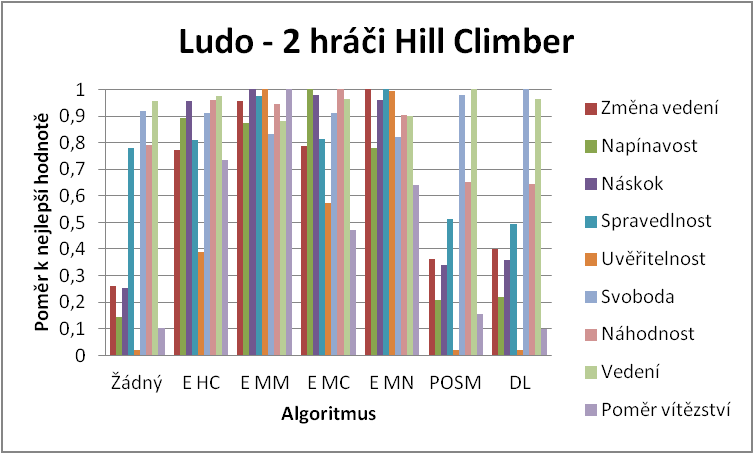
\includegraphics[width=0.90\textwidth]{ch5ludo2hc}
	\caption{popisek }
	\label{fig-ch5ludo2hc}
\end{figure}

\begin{figure}
  \centering
  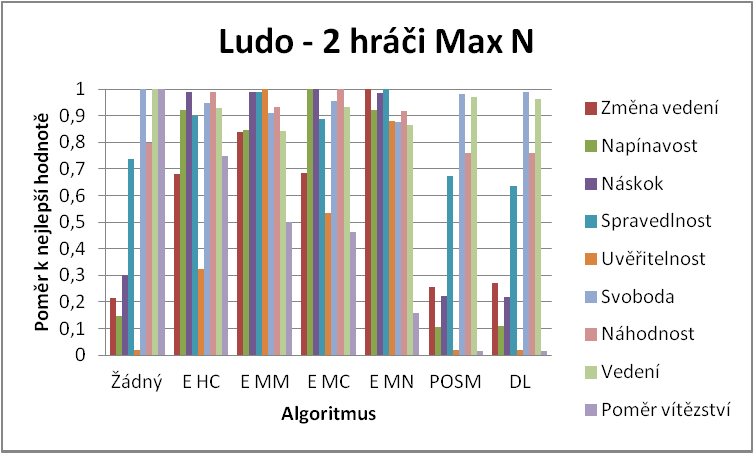
\includegraphics[width=0.90\textwidth]{ch5ludo2maxn}
	\caption{popisek }
	\label{fig-ch5ludo2maxn}
\end{figure}

\begin{figure}
  \centering
  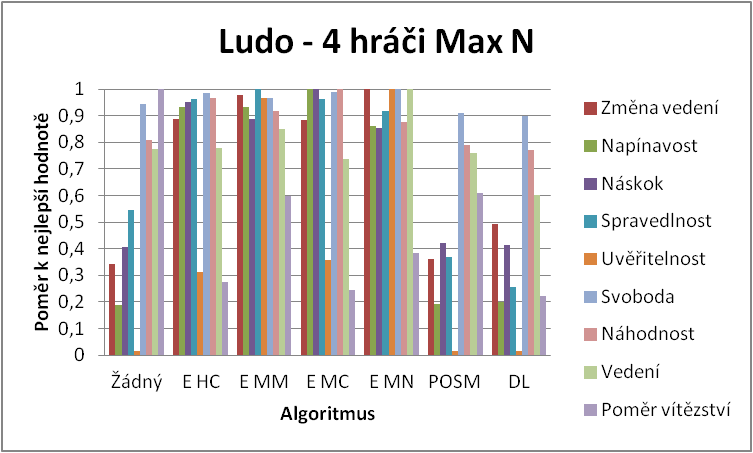
\includegraphics[width=0.90\textwidth]{ch5ludo4maxn}
	\caption{popisek }
	\label{fig-ch5ludo4maxn}
\end{figure}

\section{Ztracená města}

\begin{figure}
  \centering
  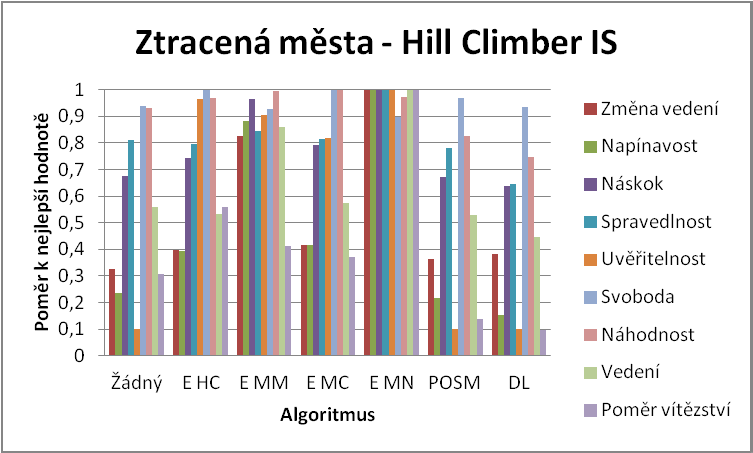
\includegraphics[width=0.90\textwidth]{ch5lchc}
	\caption{popisek }
	\label{fig-ch5lchc}
\end{figure}

\begin{figure}
  \centering
  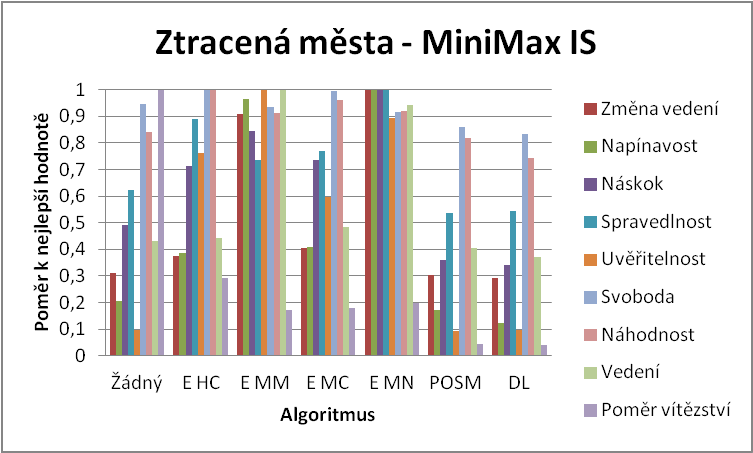
\includegraphics[width=0.90\textwidth]{ch5lcmm}
	\caption{popisek }
	\label{fig-ch5lcmm}
\end{figure}

\section{Celkové srovnání}
\begin{figure}
  \centering
  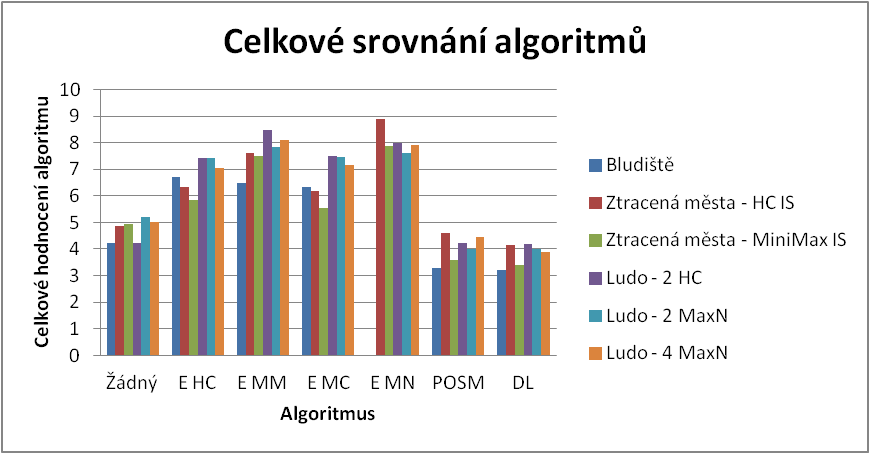
\includegraphics[width=0.90\textwidth]{ch5all}
	\caption{ popisek }
	\label{fig-ch5all}
\end{figure}

\begin{figure}
  \centering
  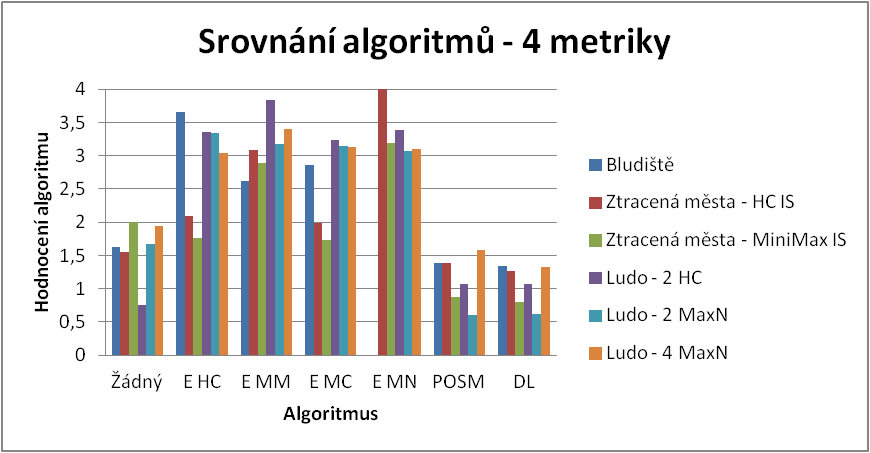
\includegraphics[width=0.90\textwidth]{ch5all4m}
	\caption{ popisek }
	\label{fig-ch5all4m}
\end{figure}

\endinput
%%
%% End of file `ch01.tex'.
